\newcommand{\Interval}{
  \begin{figure}
  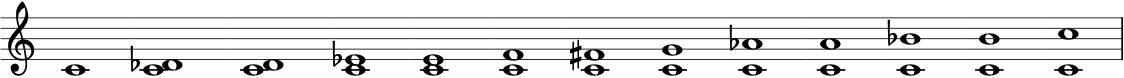
\includegraphics[width=12cm]{fig/interval.png} \\
  \begin{flushleft}
    \begin{footnotesize}
      \hspace{1.45cm} \texttt{per1 \hspace{0.5mm} min2  \hspace{2.5mm}
        maj2 \hspace{1.2mm} min3 \hspace{0.5mm} maj3 \ per4
        \hspace{1mm}aug4
        \hspace{0.5mm}  per5\hspace{1.2mm}  min6\hspace{1.6mm} maj6
        \hspace{1.6mm}min7\hspace{1.2mm} maj7\hspace{1.2mm} per8} \\
      consonant? \hspace{1.5mm} yes \hspace{4.2mm} no \hspace{6.5mm}  no
      \hspace{4.7mm} yes \hspace{3.8mm}  yes \hspace{3.7mm} no \hspace{3.5mm}
      no \hspace{4.3mm} yes \hspace{3.8mm} yes \hspace{3.2mm} yes
      \hspace{3.7mm} no \hspace{4mm} no \hspace{3.8mm} yes
    \end{footnotesize}
  \end{flushleft}
  \caption{13 Kinds of Intervals}
  \Description{13 Kinds of Intervals}
  \label{fig:interval}
 \end{figure}
}

\section{Basic Musical Terms and Their Representation in Agda}
\label{sec:music}

[TODO] Maybe need to explain degrees, instead of duration and notes.

\paragraph{Pitches}

A \emph{pitch} tells us how high or low a sound is.
We represent pitches as natural numbers, but throughout the paper,
we use a more readable notation \texttt{name octave}, where
\texttt{name} ranges over \texttt{c}, \texttt{d}, \texttt{e}, etc.,
and \texttt{octave} denotes which octave the pitch belongs to.
For instance, the middle C is represented as \texttt{c 5}.

% \begin{alltt}
% data Pitch : Set where
%   pitch : \(\mathbb{N}\) \(\rightarrow\) Pitch

% data Octave : Set where
%   octave : \(\mathbb{N}\) \(\rightarrow\) Octave

% PitchOctave : Set
% PitchOctave = Fin 12 \(\times\) Octave
% \end{alltt}

\paragraph{Duration}

\emph{Duration} denotes an unspecified unit of time during which
a sound or silence lasts.
We represent duration as a natural number, and use this value to
calculate the absolute length when the music is played at a specific
tempo.
As an example, the duration constant \texttt{whole} has value
\texttt{16} and corresponds to 4 seconds if the tempo is 60 beats
per minute.

% \begin{alltt}
% data Duration : Set where
%   duration : \(\mathbb{N}\) \(\rightarrow\) Duration
% \end{alltt}

\paragraph{Notes}

Combining pitches and duration gives us \emph{notes}.
We represent notes as a datatype \texttt{Note} with two constructors:
\texttt{tone} for notes with sound and \texttt{rest} for those without.
For example, \texttt{tone whole (c 5)} is a whole note whose sound
is the middle C.

% \begin{alltt}
% data Note : Set where
%   tone : Duration \(\rightarrow\) Pitch \(\rightarrow\) Note
%   rest : Duration         \(\rightarrow\) Note
% \end{alltt}

\paragraph{Intervals}

\Interval

An \emph{interval} represents the difference in pitch between
two notes.
There are 13 kinds of interval within an octave
(Figure~\ref{fig:interval}), and these intervals can be classified from
several different perspectives:
(i) major or minor; (ii) consonant or dissonant; and (iii) perfect
or imperfect.
We represent intervals as natural numbers, but in this paper, we
refer to them using more informative names such as \texttt{maj3}
and \texttt{per8}.

\paragraph{Chords and Triads}

A \emph{chord} refers to a set of simultaneously sounding notes.  In
this paper we are particularly interested in \emph{triads}, which are
chords consisting of three notes separated by the 3rd intervals (i.e.,
\texttt{maj3} and \texttt{min3}).  We define triads as a datatype
\texttt{Triad} with roman numeral constructors representing the scale
degree of the lowest note (called the \emph{root}). The other two
notes are then members of the scale a third and a fifth above the
root. For instance, \texttt{I} in C major represents the triad C-E-G.
